\documentclass[11pt]{article}
\title{Midterm 1 Prep}
%% Language and font encodings
\usepackage[english]{babel}
\usepackage[utf8x]{inputenc}
\usepackage[T1]{fontenc}

\usepackage{helvet}

%% Sets page size and margins
\usepackage[letterpaper,top=3cm,bottom=2cm,left=3cm,right=3cm,marginparwidth=1.75cm]{geometry}

%% Useful packages
\usepackage{amsmath}
\usepackage{graphicx}
\usepackage{tcolorbox}
\usepackage{amssymb}
\usepackage{amsthm}
\usepackage{lastpage}
\usepackage{accents}
\usepackage{multicol}

% For better list numbering
\usepackage[shortlabels]{enumitem}

% Font
% \usepackage{tgbonum}


% Tikz
\usepackage{tikz}

\usetikzlibrary{calc,fit,shapes.misc,backgrounds}
\usepackage{pgfplots}
\pgfplotsset{compat = newest}
\usetikzlibrary{positioning, arrows.meta}
\usepgfplotslibrary{fillbetween}

% Headers
\usepackage{fancyhdr}
\pagestyle{fancy}

% Store \@title as \thetitle
\makeatletter
\let\thetitle\@title
\makeatother

\fancyhf{}
\lhead{\fontfamily{qbk}\fontsize{10}{11}\selectfont ECON 3070}
\rhead{\fontfamily{qbk}\fontsize{10}{11}\selectfont \thetitle}
\rfoot{\fontfamily{qbk}\fontsize{10}{11}\selectfont \thepage}


% Sections and Subsections

% define colors
\definecolor{buff-gold}{HTML}{CFB87C}
\definecolor{buff-grey}{HTML}{565A5C}
% custom tcolorbox
\tcbset{colframe=buff-gold, colback=white!100!black}

% new page per section
\usepackage{titlesec}
\newcommand{\sectionbreak}{\clearpage}
% change style of section
\usepackage{sectsty}
\sectionfont{\color{buff-gold} \fontfamily{qbk}\selectfont}
\subsectionfont{\color{buff-grey} \fontfamily{qbk}\selectfont}


\newtoggle{INCLUDEANSWERS}
% \toggletrue{INCLUDEANSWERS}
\togglefalse{INCLUDEANSWERS}

\newcommand{\answer}[1]{\iftoggle{INCLUDEANSWERS}{{\color{violet!70!white}\textbf{Solution:} #1}}{}}


\begin{document}
  
\section*{Midterm 1 Prep}

\subsection*{Supply and Demand}
\begin{enumerate}
  \item The market for bike locks is described by the demand curve $P = 80 - Q_d$ and the supply curve $Q_s = 2P - 10 $. Answer the following questions:

    \begin{enumerate}
      \item When the price of bike locks is \$40 how many bike locks will be demanded? How many bike locks will be produced? Why would this not be the equilibrium price? Which way will the price move in this market.

      \item What is the marginal willingness to pay for the 40th bike lock? What is the marginal cost of the 40th unit?

      \item What is the market equilibrium values of price and quantity in the market of bike locks? 
    \end{enumerate}

    \answer{
      \begin{enumerate}
        \item $Q_d = 80 - P = 80 - 40 = 40$. $Q_s = 2P - 10 = 80 - 10 = 70$. This is not the equilibrium price since there is excess supply. The sellers will bid the price down.
        
        \item The marginal willingness to pay curve is given by demand, solving for $P$: $P = 80 - Q_d$. Similarly, the marginal cost curve is given by supply, solving for $P$: $P = Q_s/2 - 5$. In this case, the marginal willingness to pay is \$40 for the 40th unit and the marginal cost is \$15 for the 40th unit.
        
        \item $Q_d = 80 - P = 2P - 10 = Q_s$. This implies $3P = 90$, or $P^* = 30$. Plugging back into supply gives $Q_s = Q_d = 2*30 - 10 = 50$. Checking our work, we can plug into the demand curve and have $Q_d = 80 - 30 = 50$. 
      \end{enumerate}
    }

  \item The market contains two consumers $A$ and $B$ with the following demand functions: $Q_A^D = 40 - 5P$ and $Q_B^D = 18 - 5P$
  
  \begin{enumerate}
    \item Find the aggregate demand curve for this market. Draw this curve
    
    \answer{
      $$
        Q_{mkt}^D =
        \begin{cases}
          58 - 10P & \text{if } P \leq 4 \\
          40 - 5P & \text{if } 4 \leq P \leq 8 \\
          0       & \text{otherwise}.
        \end{cases}
      $$
    }
    
    \item Let market supply be given by $Q_{mkt}^S = 2P - 2$. Solve for the equilibrium quantity and price.
    
    \answer{
      Trying $P \leq 4$, 
      $$
        58 - 10P = 2P - 2 \implies P = 5
      $$
      This doesn't work because we assumed $P \leq 4$.

      Trying, $4 \leq P \leq 8$,
      $$
        40 - 5P = 2P - 2 \implies P = 6
      $$
      This works! Pluging back into supply, $Q_{mkt} = 2 * 6 - 2 = 10$. Checking our work, $Q_{mkt}^D = 40 - 5 * 6 = 10$. 
    }
  \end{enumerate}
\end{enumerate}

\subsection*{Supply/Demand Curve Shifters}
\begin{enumerate}
  \item For the following comparative static scenarios, describe what will happen the equilibrium price and quantity?
  
  \begin{enumerate}
    \item A stimulus check makes people richer
    \item A flood wipes out wheat crops in the midwest
    \item A flood wipes out crops in the midwest \emph{and} more people start getting into bread-making
  \end{enumerate}

  \answer{
    \begin{enumerate}
      \item Price goes up; quantity goes up
      
      \item Price goes up; quantity goes down
      
      \item Price goes up; quantity indeterminate
    \end{enumerate}
  }
\end{enumerate}


\subsection*{Elasticities}

\begin{enumerate}
  \item Suppose that when the price of the new macbook is \$1,600
  per tire, quantity demanded in Boulder is 40,000. Now suppose
  that the price has fallen to \$1,400, and the quantity demanded is
  50,000. What is the price elasticy of demand? Interpret this elasticity in words.

  \answer{
    $\% \Delta \text{ in } Q = (50,000 - 40,000) / 40,000 = 0.25$

    $\% \Delta \text{ in } P = (1,400 - 1,600) / 1,600 = -0.125$

    $$
    \frac{\% \Delta \text{ in } Q}{\% \Delta \text{ in } P} = \frac{0.25}{-0.125} = -2
    $$

    To interpret, we say a 1\% increase in price yields a 2\% decrease in quantity demanded.
  }

  \item A firm increases its price from \$8 to \$12 and sees demand for the product fall by 20\%. What would the price elasticity of demand be for this product?

  \answer{$(12 - 8)/8 = 0.5$. Therefore, $\varepsilon_{Q, P} = {0.2}{-0.5} = -0.4$. To interpret, we say that a 1\% increase in price yields a 0.4\% decrease in quantity demanded.}
  
  \item If disposable incomes rise by 5\% and demand changes from 100 units to 105, what is the income elasticity of demand? Interpret this number
  
  \answer{$(100 - 105)/100 = 5\%$. Therefore, $\varepsilon_{Q, I} = {5\%}{5\%} = 1$. To interpret, we say that a 1\% increase in income increases quantity demanded by 1\%.}
  
  \item What type of good would you expected to have a negative income elasticity of demand?
  
  \answer{Inferior good. $\frac{\partial x^*}{\partial I} < 0$}
\end{enumerate}


\subsection*{Utility Functions}
\begin{enumerate}
  \item For the following utility functions, solve for the marginal utility with respect to $x$. Interpret the marginal utility at $x = 3$. Is this utility diminishing as you increase $x$?
  \begin{enumerate}
    \item $U(x,y) = x^{1/3}y^{1/3}$
    \item $U(x,y) = 3x + 4y$
    \item $U(x,y) = x^{3/4}y^{1/4}$
  \end{enumerate}

  \answer{
    \begin{enumerate}
      \item $MU_x = 1/3 x^{-2/3} y^{1/3}$ and $MU_y = 1/3 x^{1/3} y^{-2/3}$. This is diminishing with x.
      \item $MU_x = 3$ and $MU_y = 4$. This is not diminishing with x.
      \item $MU_x = 3/4 x^{-1/4} y^{1/4}$ and $MU_y = 1/4 x^{3/4} y^{-3/4}$. This is diminishing with x.
    \end{enumerate}
  }

  \item For the following utility functions, draw two indifference curves for these utility functions. 
  \begin{enumerate}
    \item $U(x,y) = x^{1/3}y^{1/3}$
    \item $U(x,y) = 3x + 4y$
    \item $U(x,y) = x^{3/4}y^{1/4}$
  \end{enumerate}

  \item In words, describe what an indifference curve is
  
  \answer{
    The indifference curve is the set of all baskets of goods, $(x,y)$, that provide the same level of utility. Individuals (ignoring prices) are indifferent between getting given any basket on the same indifference curve.
  }
  
  \item For the following utility functions, Calculate the marginal rate of substitution $MRS_{x,y}$. Interpret the marginal rate of substitution.
  \begin{enumerate}
    \item $U(x,y) = x^{1/3}y^{1/3}$
    \item $U(x,y) = 3x + 4y$
    \item $U(x,y) = x^{3/4}y^{1/4}$
  \end{enumerate}

  \answer{
    \begin{enumerate}
      \item $MU_x = 1/3 x^{-2/3} y^{1/3}$ and $MU_y = 1/3 x^{1/3} y^{-2/3}$. 

      $$
        MRS_{x,y} = \frac{MU_x}{MU_y} = \frac{1/3 x^{-2/3} y^{1/3}}{1/3 x^{1/3} y^{-2/3}} = \frac{y}{x}
      $$

      At a point $(x,y)$, the consumer would give up 1 unit of $x$ for $\frac{y}{x}$ units of y.

      \item $MU_x = 3$ and $MU_y = 4$. 

      $$
        MRS_{x,y} = \frac{MU_x}{MU_y} = 3/4
      $$

      At a point $(x,y)$, the consumer would give up 1 unit of $x$ for $3/4$ units of y.

      \item $MU_x = 3/4 x^{-1/4} y^{1/4}$ and $MU_y = 1/4 x^{3/4} y^{-3/4}$. 

      $$
        MRS_{x,y} = \frac{MU_x}{MU_y} = \frac{3/4 x^{-1/4} y^{1/4}}{1/4 x^{3/4} y^{-3/4}} = 1/3 \frac{y}{x}
      $$

      At a point $(x,y)$, the consumer would give up 1 unit of $x$ for $1/3 \frac{y}{x}$ units of y.
    \end{enumerate}
  }  
\end{enumerate}


\subsection*{Budget Constraints}
\begin{enumerate}
  \item In words, write out the meaning of the budget constraint: 
  $$P_x x + P_y y = I$$

  \answer{The amount I spend on good $x$ plus the amount I spend on good $y$ is equal to my income.}

  \item Write out the budget constraint for $P_x = 10$, $P_y = 2$, and $I = 30$. Graph this curve.
  
  \answer{$10x + 2y = 30$}
  
  \item What happens to the above budget constraint for the following conditions:
  \begin{enumerate}
    \item $P_x$ moves to $\$5$
    \item $I$ goes up to $60$.
    \item $P_y$ drops to $\$1$.
  \end{enumerate}

  \answer{
    \begin{enumerate}
      \item The $y$-intercept stays the same at $15$, but the budget line gets more flat, intersecting the $x$ axis now at $6$ instead of $3$.
      
      \item The slope stays the same, but the $y$-intercept moves from $15$ to $30$.
      
      \item The $x$-intercept stays the same at $3$, but the budget line gets more steep, intersecting the $y$ axis now at $30$ instead of $15$.
    \end{enumerate}
  }

  \item For which of the above conditions, will the consumer be better off? How do you know? 
  
  \answer{
    Consumers are better off in all 3 scenarios because there are more goods the consumer can buy under the new budget lines.
  }
\end{enumerate}


\subsection*{Optimality Conditions}
\begin{enumerate}
  \item In words, write out why we need the optimality condition to hold for optimal consumption:
  $$
    \frac{MU_x}{P_x} = \frac{MU_y}{P_y}
  $$

  \answer{
    If the marginal utility per dollar was higher for good $x$, then you could increase utility by moving $\$1$ towards good $x$ and away from $y$. This would keep your spending constant ($+1$ and $-1$) while raising utility, thus you were not consuming optimally before. The same logic holds for good $y$.
  }

  \item For the following utility functions, write out the optimality condition
  \begin{enumerate}
    \item $U(x,y) = x^{1/3}y^{1/3}$
    \item $U(x,y) = 3x + 4y$
    \item $U(x,y) = x^{3/4}y^{1/4}$
  \end{enumerate}
  
  \answer{
    \begin{enumerate}
      \item $MU_x = 1/3 x^{-2/3} y^{1/3}$ and $MU_y = 1/3 x^{1/3} y^{-2/3}$.
      
      $$
        \frac{MU_x}{P_x} = \frac{1/3 x^{-2/3} y^{1/3}}{P_x} = \frac{1/3 x^{1/3} y^{-2/3}}{P_y} = \frac{MU_y}{P_y} 
      $$

      $$
        \implies y = \frac{P_x}{P_y} x
      $$

      \item $MU_x = 3$ and $MU_y = 4$.
      
      If $\frac{3}{P_x} > \frac{4}{P_y}$, consume $x$ only. If $\frac{3}{P_x} \leq \frac{4}{P_y}$, consume $y$ only.

      \item $MU_x = 3/4 x^{-1/4} y^{1/4}$ and $MU_y = 1/4 x^{3/4} y^{-3/4}$.
      
      $$
        \frac{MU_x}{P_x} = \frac{3/4 x^{-1/4} y^{1/4}}{P_x} = \frac{1/4 x^{3/4} y^{-3/4}}{P_y} = \frac{MU_y}{P_y} 
      $$

      $$
        \implies y = \frac{P_x}{3P_y} x
      $$
    \end{enumerate}
  }

  \item Write out the three main utility functions we have talked about in class. What are the optimality conditions for each of them?
  
  \answer{
    \begin{enumerate}
      \item Cobb-Douglas: $U(x,y) = x^{\alpha} y^{\beta}$. The optimality condition is:
      
      $$
        y = \frac{\beta}{\alpha} \frac{P_x}{P_y} x
      $$

      \item Perfect Substitutes: $U(x,y) = ax + by$. The optimality condition is:
      
      If $\frac{a}{P_x} > \frac{b}{P_y}$, consume $x$ only. If $\frac{a}{P_x} \leq \frac{b}{P_y}$, consume $y$ only.

      \item Perfect complements: $U(x,y) = \min(ax, by)$. The optimality condition is:
      
      Consume $ax = by$.
    \end{enumerate}
  }
\end{enumerate}


\subsection*{Optimal Demand}
\begin{enumerate}
  \item Interpret in words the optimization problem that consumers face:
  $$
    \max_{x,y} U(x,y) \text{ subject to } P_x x + P_y y = I
  $$

  \answer{Maximize the objective function, the consumer's utility, given the constraint of their budget.}

  \item What are the two things you need to solve for optimal demand?

  \answer{The optimality condition and the budget constraint.}

  \item Solve the following problems for demand

  \begin{enumerate}
    \item $U(x,y) = \min(2x, y) \text{ and } P_x = 3, P_y = 1, I = 20$
    
    \item $U(x,y) = 2x + y \text{ and } P_x = 1, P_y = 3, I = 24$
    
    \item $U(x,y) = x^{\frac{2}{3}} y^{\frac{1}{3}}  \text{ and } P_x = 2, P_y = 2, I = 18$
  \end{enumerate}

  \answer{
    \begin{enumerate}
      \item The budget constraint is $3x + y = 20$. The optimality condition is $2x = y$. 
      
      Plugging in the optimality condition to the budget constraint yields $3x + 2x = 20 \implies x^* = 4$. Plugging this back into the optimality condition yields $2 * 4 = y^* = 8$.

      \item $MU_x/P_x = 2/1 = 2$. $MU_y / P_y = 1/3$. Consume only $x$ which implies $y^* = 0$ and $x^* = I/P_x = 24/1 = 24$.
      
      \item The optimality condition is $y = \frac{2/3}{1/3} \frac{1}{3} x = 2/3x$. The budget constraint is $2x + 2y = 18$. 
      
      Plugging in the optimality condition to the budget constraint yields $2x + 2 (2/3x) = 18 \implies x^* = 5.4$. Plugging this back in yields $y^* = 2/3 * 5.4 = 3.6$.
    \end{enumerate}
  }
\end{enumerate}

\subsection*{Consumption Curves}
\begin{enumerate}
  \item Solve for the demand functions $x^*(P_x, P_y, I)$ and $y^*(P_x, P_y, I)$ for the following utility functions:
  
  \begin{enumerate}
    \item $U(x,y) = x^{1/2} y^{1/2}$
    \item $U(x,y) = \min(x, 2y)$
    \item $U(x,y) = 2(x + y)$
  \end{enumerate}

  \answer{
    \begin{enumerate}
      \item The optimality condition is $y = P_x/P_y x$. The budget constraint is $P_x x + P_y y = I$. Plugging the optimality condition in yields:
      $$
        P_x x + P_y (P_x/P_y x) = I \implies x^* = \frac{I}{2P_x}.
      $$
      Similarly, $y^* = \frac{I}{2P_y}$.

      \item The optimality condition is $x = 2y$. The budget constraint is $P_x x + P_y y = I$. Plugging the optimality condition in yields:
      $$
        P_x 2y + P_y y = I \implies (2P_x + P_y)x = I \implies x^* = \frac{I}{2P_x + P_y}
      $$

      \item $\frac{MU_x}{P_x} = \frac{2}{P_x}$. $\frac{MU_y}{P_y} = \frac{2}{P_y}$. If $\frac{MU_x}{P_x} > \frac{MU_y}{P_y}$, consume only $x$. Similarly, if $\frac{MU_x}{P_x} \leq \frac{MU_y}{P_y}$, consume only $y$.
      
      As an aside, $\frac{MU_x}{P_x} > \frac{MU_y}{P_y}$ is equivalent to $P_y > P_x$. Likewise, $\frac{MU_x}{P_x} \geq \frac{MU_y}{P_y}$ is equivalent to $P_x \geq P_y$. Therefore, if $P_y > P_x$, consume only $x$ and if $P_y \leq P_x$, consume only $y$.
    \end{enumerate}
  }


  \item Solve for the demand functions $x^*(P_x, P_y, I)$ and $y^*(P_x, P_y, I)$ for $U(x,y) = x^{1/2} y^{1/2}$. Answer the following
  \begin{enumerate}
    \item What is the deriviative with respect to income, $I$? Does this imply the good is a normal good or a inferior good?
    
    \item Do $x$ and $y$ satisfy the law of demand
    
    \item Graph the demand curve $x^*(P_x)$ for $I = 12$ and $P_y = 4$ with $P_x$ on the $y$-axis and $x^*$ on the $x$-axis.
    
    \item Graph the engel curve $x^*(I)$ for $P_x = 4$ and $P_y = 2$ with $I$ on the $y$-axis and $x^*$ on the $x$-axis.
  \end{enumerate}

  \answer{
    From above, $x^* = \frac{I}{2P_x}$ and $y^* = \frac{I}{2P_y}$
    \begin{enumerate}
      \item $\partial x^* / \partial I = \frac{1}{2P_x} > 0$. This is a normal good. $\partial y^* / \partial I = \frac{1}{2P_y} > 0$. This is a normal  good as well.
      
      \item Yes. $\partial x^* / \partial P_x < 0$ and $\partial y^* / \partial P_y < 0$.
      
      \item The demand curve is given by $x^*(P_x) = 12/P_x$. Solving for $P_x = 12/x^*$. Plot this.
      
      \item The engel curve is given by $x^*(P_x) = I/4$. Solving for $I = 4/x^*$. Plot this.
    \end{enumerate}
  }
\end{enumerate}

\subsection*{Income and Substitution Effect}
\begin{enumerate}
  \item In words, describe what the income effect and the substitution effects are.
  
  \answer{The income and substitution effects transfer decomposes the total effect of a price change. The substitution effect says, holding fixed utility level, when good $x$ becomes less expensive, $MU_x/P_x$ increases, shifting consumption towards good $x$. The income effect says when $P_x$ goes down, your effective income goes up, so you buy more/less of a good depending on if it is a normal or inferior good.}
  
  \item Suppose that the price for good $x$ increases, show using the optimality condition, why you know that demand for $x$ must decrease. 
  
  \answer{$MU_x / P_x$ decreases since $P_x$ increases. Hence, $MU_y / P_y > MU_x / P_x$ and consumption must move towards $y$ and away from $x$.}
  
  \item How do you know if the income effect is positive or negative?
  
  \answer{If the good is a normal good or an inferior good.}

  \item For the below figure, highlight the income effect and the substitution effect. Is this good a normal good or an inferior good?
  
  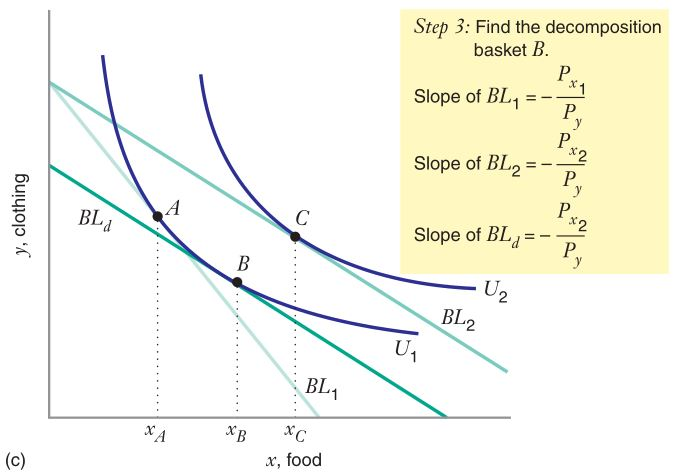
\includegraphics[width=0.6\linewidth]{../Lecture Slides/figures/fig5_6c.JPG}

  \answer{
    Substitution effect: $A \rightarrow B$
    
    Income effect: $B \rightarrow C$

    Since the income effect is positive for $x$ and for $y$, both goods are normal goods.
  }
\end{enumerate}

\subsection*{Consumer Welfare}
\begin{enumerate}
  \item If the demand for a product is $Q_D = 100 - 4P$, what is the consumer surplus generated when the market price is $P = 10$? Suppose a tax is imposed that raises the equilibrium price to $P = 12$. What is the new consumer surplus? What is the loss in consumer surplus from this tax?
  
  \answer{Solving for $P = 25 - Q/4$. The consumer surplus triangle has the points $(0, 10)$, $(0, 25)$ and $Q = 100 - 4 * 10 = 60 \implies$ $(60, 10)$. The area is thus $C.S. = 1/2 * 60 * (25 - 10) = 450$. 
  
  At the new price, the consumer surplus triangle has the points $(0, 12)$, $(0, 25)$ and  $Q = 100 - 4 * 12 = 52 \implies$ $(52, 12)$. Thus the area is $C.S._{new} = 1/2 * 52 * (25 - 12) = 338$. Consumer surplus went down by $112$.}

  \item If the demand for a product is $Q_D = 144 - 12P$, what is the consumer surplus generated when the market price is $P = 6$? Suppose a subsidy is imposed that lowers the equilibrium price to $P = 4$. What is the new consumer surplus? What is the gains for consumers from this subsidy?
  
  \answer{Solving for $P = 12 - Q/12$. The consumer surplus triangle has the points $(0, 6)$, $(0, 12)$ and $Q = 144 - 12 * 6 = 72 \implies$ $(72, 6)$. The area is thus $C.S. = 1/2 * 72 * (12 - 6) = 216$. 
  
  At the new price, the consumer surplus triangle has the points $(0, 4)$, $(0, 12)$ and  $Q = 144 - 12 * 4 = 96 \implies$ $(96, 4)$. Thus the area is $C.S._{new} = 1/2 * 96 * (12 - 4) = 384$. Consumer surplus went up by $168$.}
\end{enumerate}

\subsection*{Labor-Leisure}
\begin{enumerate}
  \item The current wage in Boulder is $12$. The consumer's utility function for labor, $L$, and the composite good $Y$ is given by $U(L, Y) = L^{1/2} Y^{1/2}$. 
  
  \begin{enumerate}
    \item Write out the budget constraint for leisure and the composite good.
    
    \item Solve for this consumer's optimal amount of hours worked, $24 - L$, and the amount of the composite good, $Y$, they consume.
    
    \item Now, suppose a minimum wage increases wages to $15$. Solve for hours worked and the amount of the composite good consumed.
  \end{enumerate}

  \answer{
    \begin{enumerate}
      \item $24w = wL + Y \implies 288 = 12L + Y$
      
      \item The optimality condition is:
      $$
        \frac{MU_L}{w} = \frac{MU_y}{1} \implies \frac{1/2 L^{-1/2} Y^{1/2}}{w} = 1/2 L^{1/2} Y^{-1/2} \implies Y = wL
      $$

      In this case, the optimality condition is $Y = 12L$. Plugging this into the budget constraint yields
      $$
        288 = 12L + 12L \implies L^* = 288/24 = 12
      $$
      Therefore, the number of hours worked is $24 - 12 = 12$. Plugging $L^*$ into the budget constraint yields $288 = 12 * 12 + Y \implies Y^* = 144$.

      \item The new optimality condition is $Y = 15L$. Plugging this into the budget constraint yields
      $$
        288 = 12L + 15L \implies L^* = 288/27 = 10.66
      $$
      Therefore, the number of hours worked is $24 - 10.66 = 13.34$. Plugging $L^*$ into the budget constraint yields $288 = 15 * 10.66 + Y \implies Y^* = 128$.

    \end{enumerate}
  }

  \item Say that the wage raised from \$15 to \$20 and the amount of labor supplied decreases. Explain why that could be possible.

  \answer{
    Since leisure is now relatively more expensive, the consumer's substitution effect would be away from leisure (towards working). However, the income effect (that you make more money from working) could be negative. The income effect would have to be larger than the substitution effect to lower the labor supply. 
  }
\end{enumerate}


\end{document}
